\documentclass[11pt,letterpaper,english]{article}
\usepackage[T1]{fontenc} % Standard package for selecting font encodings
\usepackage{txfonts} % makes spacing between characters space correctly
\usepackage{xcolor} % Driver-independent color extensions for LaTeX and pdfLaTeX.
\usepackage{hyperref}  %The ability to create hyperlinks within the document

\usepackage{fancyhdr} % header footer placement

\usepackage[top=1in, bottom=1in, left=1in, right=1in] {geometry} % Margins
\usepackage{graphicx}   % Essential for adding images to you document.

\usepackage[numbers]{natbib}

%\usepackage{sectsty}
%% \sectionfont{\normalsize}
%% \subsectionfont{\normalsize}
%\subsubsectionfont{\normalsize \it}

\usepackage[small,compact]{titlesec}
\titlespacing{\section}{0pt}{0.5em}{0.25em}
\titlespacing{\subsection}{0pt}{0.5em}{0.125em}
\titlespacing{\subsubsection}{0pt}{0.5em}{0.25em}
\titlespacing{\paragraph}{0pt}{0.75em}{0.25em}

\setlength{\textfloatsep}{7pt}

\titleformat*{\subsubsection}{\itshape}

\let\oldthebibliography=\thebibliography
  \let\endoldthebibliography=\endthebibliography
  \renewenvironment{thebibliography}[1]{%
    \begin{oldthebibliography}{#1}%
      \setlength{\parskip}{0.1ex}% 
      \setlength{\itemsep}{0.0ex}% 
  }%
  {% 
    \end{oldthebibliography}% 
  }


% commas between multiple footnotes
\newcommand\fnsep{\textsuperscript{,}}

\usepackage{caption}
\captionsetup{labelsep=period}

\setlength{\parskip}{0.1\baselineskip}%
%\setlength{\parindent}{0pt}%

\input newcommands

%\raggedright

\begin{document}

\pagestyle{fancy} 
\lhead{Approaching Exascale Models of Astrophysical Explosions} 
\rhead{PI: Zingale} \renewcommand{%
\headrulewidth}{0.0pt}

\begin{center}
{\bf PROJECT NARRATIVE}
\end{center}


%-----------------------------------------------------------------------------
\section{SIGNIFICANCE OF RESEARCH}

%% Explain what advances you expect to be enabled by an INCITE award that
%% justifies an allocation of petascale resources (e.g., anticipated
%% impact on community paradigms, valuable insights into or solving a
%% long-standing challenge, etc). Place the proposed research in the
%% context of competing work in your discipline or business. The
%% information should be sufficient for peer review in your area of
%% research and also appropriate for general scientific review comparing
%% your proposal with proposals in other disciplines. Potential impact is
%% the predominant determinant for awards. This factor will be assessed
%% by a peer-review panel. Also list any previous INCITE award(s)
%% received and discuss the relationship to the work proposed. {\bf This
%%   section is typically about 4 pages.}

We propose a collaborative investigation of multiple types of stellar
explosions and their precursors using a suite of state-of-the-art
hydrodynamics codes.  Several progenitor models of Type Ia supernovae
will be explored, including their pre-explosion and explosive phases,
using our codes \maestro, \castro, and \flash.  X-ray bursts will also
be studied in their pre-explosive and explosive phases, using
\maestro\ and \castro.  The curious radiation-dominated systems like
the black widow pulsar will be explored with \castro, and
core-collapse supernovae will be studied using \chimera.  All
calculations will be three-dimensional and face the challenges of
capturing the effects of turbulence, instabilities, strong
gravitational interactions, nuclear reactions, and radiation.  These
challenges make these problems INCITE-class, and only the resouces
titan can provide will enable use to further our understanding.
Despite the broad suite of codes, there are common links, namely in
the microphysics (reactions, equations of state) and in our shared
approach to utilitizing the GPUs on titan.  This collaboration is an
expansion of our existing INCITE proposal, but we believe that it
represents the most efficient use of resources, allowing us to work
together as a team to create portable solvers to effectively make
use of this architecture and its successor.  These GPU-enabled
solvers will be made freely available.

Our publication record demonstrates that we have made productive use
of our current INCITE award, and we expect similar productivity
carrying forward.  Furthermore, this INCITE time will be used to train
the next generation of computational scientists---graduate students
feature prominently in the proposed work plan.


\subsection{Type Ia supernovae}

Type Ia supernovae (SNe Ia) are the thermonuclear explosion of a
carbon/oxygen white dwarf (WD) in a binary system.  These are incredibly
bright explosions that rival the light output of their host galaxy,
making them visible at vast distances in the Universe.  Furthermore,
they have an interesting property: the brightest events take the
longest to dim.  This allows them to be used as distance indicators
and led to the discovery of the acceleration of the expansion of the
Universe~\cite{Per99,Rie98} (recently awarded the Nobel Prize).

A fundamental uncertainty in our understanding of SNe Ia is the nature
of the progenitor---a single white dwarf accreting from a normal
companion star (single degenerate scenario) or two white dwarfs that
inspiral (or violently collide) and merge (the double degenerate
scenario).  No progenitor system of an SN Ia has ever been
identified, so astronomers must look for indirect clues.  Regardless
of the progenitor system, in every case the majority of the carbon and
oxygen in the white dwarf(s) is converted into iron/nickel and
intermediate-mass elements like silicon, and this nuclear energy
release unbinds the star.

For many years, the Chandrasekhar-mass single degenerate model
(henceforth called the Chandra model) saw the most attention.  The
Chandrasekhar mass is the maximum possible mass of a white
dwarf---beyond this mass, the degenerate electrons that provide the
pressure support against gravity in a white dwarf succumb to the
weight of the star and it will collapse into an even more dense
object: a neutron star.  By always exploding near the Chandrasekhar
mass, the same amount of fuel will be involved in every event and to
first-order all SNe Ia would be alike.  Many groups
(e.g.~\cite{gamezo:2005,Roe07,Jor08}, including us~\cite{Kru12,Ma13})
have modeled the explosion (and also the convective stage
preceding it~\cite{hoflichstein:2002}; again including us~\cite{Non12}) and have shown that it can reproduce the
spectra and lightcurves of the observations~(e.g.~\cite{Blo11}).
However, it is not clear if nature makes SNe Ia this way---massive
carbon/oxygen white dwarfs in binary systems are rare.  An additional
complication is that the successful models rely on a
deflagration-to-detonation transition (subsonic to supersonic
burning), the physics of which is not completely understood.  Buoyed by
observations that showed SNe Ia are more diverse than previously
thought, and evidence that there may be two
populations~\cite{MannucciEtAl06,howelletal+09,How11}, two
alternative models, the double
degenerate and sub-Chandra models for SNe Ia, have become more
scientifically interesting.  Theoretically, these both have
challenges.

The standard picture for double degenerate SN Ia (henceforth WDWD) has the
two white dwarfs spiraling toward each other as gravitational radiation
removes orbital energy from the system.  Here the white dwarfs can be more
moderate in mass, but the sum of their masses may exceed the
Chandrasekhar mass.  As the stars inspiral, the less massive star will
become tidally disrupted and the more massive star will accrete this
material.  A longstanding concern is that when this mass transfer
begins, thermonuclear burning can ignite at the edge of the star,
converting it to oxygen/neon/magnesium, and leading to the collapse of
the white dwarf into a neutron
star~\cite{saionomoto:2004,fryerdiehl:2008}, instead of an SNe Ia.
This system is inherently three-dimensional, and only through detailed
simulation can we understand the dynamics of the mass transfer, and
thereby assess the feasibility of this model.  Alternatives involving
(nearly) head-on collisions of white dwarfs may account for a few
events, but are unlikely to explain the majority.

The other alternative mechanism, sub-Chandra mass single degenerate SNe
Ia~\cite{fink:2010,shen:2010,sim:2012} (henceforth called the sub-Ch
model), has the advantage that systems with a moderate mass white dwarf
(0.8--1.0 solar masses) are known and abundant.  In addition, they are
able to reproduce what we know of delay-time distributions and SNe Ia
rates---something the Chandra model struggles with~\cite{ruiter:2011}.
The core idea of this model is that the white dwarf accretes a layer
of helium on its surface and a detonation ignites in this helium
layer.  This surface detonation can send a compression wave into the
underlying carbon/oxygen white dwarf, compressing the core to the point 
of igniting a detonation that unbinds the star. The main
problem with this ``double detonation'' 
model is that it is easier to ignite a detonation in
a more massive helium layer than a low mass helium layer, but too much
helium will lead to excessive production of iron-group elements when
compared to observations. Also, 
models have difficulty reproducing the intermediate mass elements 
(i.e.\ Si) seen in the spectra on standard SNe
Ia~\cite{hoeflich:1996,nugent:1997,kromer:2010}.  
Investigations into 
so-called ``.Ia'' explosions suggest the mass of the helium shell need
not be as large as previously assumed to trigger
runaway~\cite{bildsten:2007}.  Inspired by this, it has been suggested
that a detonation in a very thin He layer can trigger the detonation
of the core without over-producing surface iron-group
elements~\cite{fink:2010}, although detailed 1D stellar evolution
calculations suggest that these smallest mass He shells may ignite as
deflagrations or novae instead of as detonations, depending on the
properties of the system~\cite{woosleykasen:2010}.  If it can ignite
as a detonation, synthetic lightcurves can match
observations~\cite{kromer:2010}.  The challenge now becomes
understanding whether and under what conditions ignition can take
place in these thin shells when a realistic 3D convective field is
realized, as well as the subsequent evolution and character of that
ignition---this is what we will answer.

In past INCITE awards, we focused on the last hours of
convection, ignition, and the explosion in the Chandra model.  There
is an aspect of the Chandra model that we have not explored in
detail---this is the earliest stages of the convection in the white
dwarf, when neutrino losses in the reaction can alter the dynamics of
the convection (called the URCA process).  The only multi-dimensional
simulations of URCA~\cite{URCA} to date have been 2D, with only a
portion of the star modeled.  We can apply the same methodology we
used for the ignition calculations in the Chandra model during our
current INCITE award to study this problem in 3D.  This will be a
small focus of the proposed work.



\subsection{Type I X-ray bursts}

Type I X-ray bursts (XRBs) are the thermonuclear runaway of a thin
layer of hydrogen and/or helium on the surface of a neutron star. 
This fuel layer accretes from a binary companion star and the immense
gravitational acceleration on the surface of the neutron star
compresses it, increasing the temperature and density to the point of
explosion.  One-dimensional hydrodynamic studies have been able to
reproduce many of the observable features of XRBs such as burst
energies ($\sim 10^{39}$ erg), rise times (seconds), durations ($10$'s
-- $100$'s of seconds) and recurrence times (hours to days) (see
\cite{STRO_BILD06} for an overview of XRBs).  By construction,
however, 1D models assume that the fuel is burned
uniformly over the surface of the star which is unlikely if the
accretion is not spherically symmetric \cite{SHARA82}.  Furthermore,
the {\em Rossi X-ray Timing Explorer} satellite has observed coherent
oscillations in the lightcurves of $\gtrsim 20$ outbursts from low-mass
X-ray binary
systems (first by \cite{STRO_ETAL96}; more recently by
\cite{ALTAMIRANO_ETAL10} and references therein).  The asymptotic
evolution of the frequency of such oscillations suggests they are
modulated by the neutron star spin frequency \cite{MUNO_ETAL02} and
are therefore indicative of a spreading burning front being brought in
and out of view by stellar rotation.

Before the actual outburst, the burning at the base of the ignition
column will drive convection throughout the overlying layers and set
the state of the material in which the burning front will propagate.
One-dimensional simulations of XRBs usually attempt to parametrize the
convective overturn and mixing using astrophysical mixing-length
theory or through various diffusive processes
(e.g. \cite{HEGER_ETAL00}).  A proper treatment of the convection in
these extreme conditions, free from parameterizations, requires 3D
simulations.  We completed the most detailed (2D) studies of
convection in pure He bursts~\cite{XRB-paper} and mixed H/He
bursts~\cite{XRB2}, and have just begun 3D simulations.  3D is
expensive, restricting us to small domains to resolve the burning
processes and small reaction networks (10-isotopes currently) to fit
the model in memory.  In small domains, the convection ``senses'' 
the boundaries, which can alter the dynamics.  Ultimately we want
to model a wide domain with many convective plumes side-by-side
and a more realistic reaction network---this is what we will
accomplish with our proposed simulations.


\subsection{\maestro\ and \castro}

The workhorses of the proposed work will be our state-of-the-art
simulation codes \maestro~\cite{multilevel} and
\castro~\cite{castro:I}, developed over the past 8 years in
collaboration with Lawrence Berkeley Lab.  \maestro\ is tuned to
efficiently model the highly subsonic convective flows that often
precede stellar explosions.  It accomplishes this by reformulating
the equations of hydrodynamics, filtering the
soundwaves from the equations of hydrodynamics, while keeping 
the compressibility effects due to stratification and local heat release.
\maestro\ has been used successfully to model the convection leading
to ignition in the Chandra model for SNe Ia (a focus of our current
INCITE allocation) and will continue to be used for the XRB and sub-Ch
convection simulations proposed here.  \castro\ solves the fully
compressible equations of hydrodynamics, allowing it to model shocks
and explosive phenomena.  It will be the simulation code for the white
dwarf merger simulations, and in later years, for the explosions
following the convection phases modeled by \maestro.  \maestro\ and
\castro\ share the underlying microphysics e.g., equation of state
(EOS) and nuclear reaction networks, as well as the underlying
\boxlib\ library that manages their adaptive mesh refinement (AMR)
grid hierarchy.  This makes it straightforward to transition a problem
from \maestro\ to \castro, as was done during our current INCITE
allocation when studying flame propagation in Chandra model SNe
Ia~\cite{Mal14}.  Both codes are already up and running on our target
platform, titan (OLCF).  Additionally, both codes are publicly
available%
\footnote{\maestro: \url{http://bender.astro.sunysb.edu/Maestro/}}\fnsep\footnote{\castro: \url{https://ccse.lbl.gov/Downloads/downloadCASTRO.html}}---any
performance or physics improvements developed under this INCITE award
will become part of the public releases, benefiting the community
at large.


\subsection{Core-collapse supernovae}



\subsection{Work under previous INCITE awards}

We are currently in the last year of a 2-year INCITE award (AST106;
PI: Zingale; allocation on OLCF/titan) that focused on XRBs and SNe
Ia.  Many of the current investigators have also collaborated on other
previous INCITE awards.  \MarginPar{number of papers}

{\bf \maestro\ convection models}:
%
We completed our initial study of sub-Ch SNe Ia
simulations~\cite{Zin13} with \maestro, and are currently writing up
the results of our second study (led by graduate student co-I Jacobs).
These are the only models in the world that have explored the dynamics
of the convection in the accreted helium layer in a full-3D resolved
simulation.  This study showed that \maestro\ presents a robust
simulation platform for investigating the physics of ignition in the
accreted helium layer.  Follow-on calculations have explored a range
of WD and He-shell masses and what minimum mass is necessary for
ignition.  A paper describing these results is in preparation.

An original focus of our INCITE award was modeling the convection in
Chandra mass white dwarfs leading up to an SNe Ia.  This has been
completed and published in a series of
papers in the Astrophysical Journal~\cite{Zingale:2011,Non12}.  We
used AMR to greatly increase the resolution of
our ignition simulations---this allowed us to explore the resolution
dependence of our results.  We demonstrated that the ignition is most
likely to take place off-center, around 50~km from the center of the
white dwarf, and by following hotspots as they develop in the flow, we
showed that ignition is likely only at a single point.  We
characterized the turbulence in the convective region and showed that
it follows Kolmogorov statistics.  Further, we measured its intensity
and integral length scale and argued that it is unlikely to affect the
flame propagation.

Finally, we did the first simulation using \maestro\ convection
results for a Chandra model SN Ia as initial conditions in \castro\ to
model the subsequent explosion~\cite{Mal14}.  This ``end-to-end''
capability is facilitated by the fact that the two codes share the
same underlying \boxlib\ library.  This is the first 3D calculation of the 
explosion phase in the 
literature to begin with a self-consistent convective field.  This capability added to our understanding
of how the convection affects the evolution of the explosion.  One of
the results from this study was that the flame is unhindered by
turbulent convection for typical ignition locations ($\sim 40$ km
off-center), but is strongly distorted for more centrally-located
ignition.  Even a perfect sphere ignited at the center of the star
will be carried off-center by the turbulent convection.  This results
in asymmetric explosions for all Chandra models, which should be
accounted for when matching to observations.

{\bf \castro\ WD merger models}:
%
A final focus of research under our current INCITE award, begun only
recently, are the initial simulations of the WDWD problem.  \castro\ had not yet been deployed for problems of this type,
and therefore required a number of algorithmic
improvements, including new boundary conditions for the gravity solver
and better treatment of the temperature in the hydrodynamics module.
Titan was used for verification purposes by running simulations of the
early part of a merger scenario, when the two WDs are orbiting each
other at a large distance. In this case, the motion should remain
stable, and as with all hydrodynamics codes, conservation of energy
and angular momentum was paramount. We performed several large-scale
simulations of these, checking various parts of the parameter space to
ensure that we can robustly simulate these events. This helped us fix
a number of underlying issues, and we are beginning production runs.
We note that these calculations are different than those lead by the
UCSC/UCB group above---they started with a merged remnant and then
modeled the subsequent explosion.  In the work proposed here, we 
will model the merger process itself.  This project is led by graduate
student co-I Katz.


\subsection{Significance of our proposed work}

To advance the state of the knowledge of SNe Ia and XRBs, we will
carry out the following sets of simulations (all in 3D):
\begin{tightitem}
\item Full star \maestro\ sub-Ch models with 
  detailed nucleosynthesis and realistic initial models.
\item \castro\ sub-Ch explosion models beginning with the
  \maestro\ initial conditions.
\item The largest-domain-to-date 3D resolved \maestro\ XRB convection
  calculations.
\item The first XRB convection calculations with a burning sub-grid
  model.
\item Highly-resolved \castro\ WDWD models capturing multiple orbits
  and the inspiral.
\end{tightitem}

We are the only group in the world modeling the detailed convection
with realistic nuclear physics in XRBs and the sub-Ch SNe Ia.
In all simulations we will push the size of the nuclear reaction networks
to accurately capture the nucleosynthesis (as discussed later, GPUs will
be used for this task).

XRBs are important probes of the nuclear equation of
state~\cite{ozel:2010,steiner:2010}, and the nucleosynthesis that
takes place will involve the nuclei that are a target of the DOE FRIB
experiment.  Our simulations will advance our understanding on the
burning dynamics and tell us (1) whether any burning products can be
carried to the photosphere, altering the interpretation of
observations; (2) how the full 3D treatment of convection modifies the
nucleosythesis, allowing us to provide feedback to the 1D modelers;
(3) how to create a sub-grid model to enable larger scale simulations;
and (4) ultimately, in year 3 when we are able to implement a sub-grid
model, start to learn how turbulence in the burning alters the
spreading of the front across the neutron star.  With \maestro, we are
in the unique position to address each of these points.

While several groups are investigating explosions in the sub-Ch model,
we are the only group that is modeling the 3D convective field and
ignition that precedes the explosion.  Much like our previous INCITE
work in carrying \maestro\ convection calculations of the Chandra
model into the explosion phase with \castro, our similar work here
(proposed for year 3) for the sub-Ch model will be unmatched.
Initially we will focus on using more realistic models of WDs
generated from stellar evolution codes (we currently use simple
parametrized models), and we will answer the question of which
configurations (WD mass and He mass) lead to ignitions as well as the
timing and geometry of this ignition.  Along the way we will switch
from our simplified 4-isotope network to a more general in-situ
network to better understand the sensitivity of our results to the
nuclear physics, metallicity, and trace abundances of other species.
In addition, we will complete our implementation of nucleosynthetic
post-processing using Lagrangian tracer particles to allow offline
exploration.  This is key, as the exact composition of the helium
layer at detonation can have profound effects on the subsequent
observations, impacting the model's viability as a SNe Ia
progenitor~\cite{kromer:2010}.  All simulations will be 3D, and the
vast majority will model the entire star.  These results will provide
the foundation for \castro\ simulations capable of determining if the
ignition evolves as a detonation and that detonation's subsequent
evolution with realistic 3D initial conditions.
 
Several groups are pursuing WDWD
mergers~\cite{yoon:2007,motl:2007,loren-aguilar:2009,shenetal+11} or
collisions~\cite{raskinetal+10,loren-aguilar:2010,rosswog:2009}. The
majority of these have used smoothed particle hydrodynamics (SPH), a
gridless alternative to the methods we use here.  SPH is known to have
trouble capturing instabilities and has low resolution in regions of
low density---precisely the regions where the stars make contact.  Our
grid--based simulations will provide an important counterpart to
existing simulations.  With the power of AMR, we can push far beyond
the resolutions of the grid-based simulations in the current
literature to levels necessary to assess whether an explosion upon
contact is feasible. \castro\ is ready for these simulations---we have
made the necessary changes for isolated gravity boundary conditions,
and while we will start with simple WD models on the grid, we are
nearly complete in implementing a self-consistent method to initialize a binary
pair of WDs on our grid using the full stellar equation of state.



%-----------------------------------------------------------------------------
\section{RESEARCH OBJECTIVES AND MILESTONES }  

%% Describe the proposed research, including its goals, milestones and
%% the theoretical and computational methods it employs. Goals and
%% milestones should articulate simulation and developmental objectives
%% and be sufficiently detailed to assess the progress of the project for
%% each year of any allocation granted. Milestones should correlate with
%% those in the milestone table. It is especially important that you
%% provide clear connections between the project's overarching
%% milestones, the planned production simulations, and the compute time
%% expected to be required for these simulations (e.g., should correlate
%% with those in the ``Use of Resources Requested'' section below). {\bf
%%   This section is typically about 6 pages.}

As described above, we plan a suite of comprehensive simulations of
XRBs and SNe Ia (both the sub-Ch and WDWD models) using our
codes \maestro\ and \castro.  All the problems we
describe are inherently three-dimensional, requiring large resources.
Our codes are running on titan today, and they perform and scale
well.  The starting point for all the simulations proposed are in
place.  We are ready to run.

The calculations we describe in further detail here are INCITE--class
for two reasons.  First, as is often the case in astrophysics, we can
never capture all the length-scales that come into play in these
stellar explosions, for example, the turbulent dissipation scale in
the convective regions is often quite below our grid resolution.  As a
result, we need to push to higher-and-higher resolution to assess
whether our results are converged.  This high resolution demands a lot
of computational resources---the type that only INCITE can provide.
Second, the temporal scales we need to model are equally impressive.
For the XRB simulations, we would like to model a second of evolution.
At our current resolution (6~cm), we would need over a million
timesteps (and that is with the large efficiency gain we get through
the low Mach model).  Since there is no parallel-in-time equivalent to
domain decomposition, we need to run a big problem for long amounts of
time on the machine---again, a feat only possible through INCITE.
Finally, we want to push the realism of the physics, in particular,
our reaction networks.  This will only be feasible by offloading some
of the reaction expense to the GPUs.

The basic motivation for our science problems was given in the
previous section.  Here we begin by discussing the milestones we hope
to achieve in each year and then we give specific details about the
number and size of the simulations we plan to run.  We note that because
we have preliminary calculations of each of the problems we propose to
run, we can base our time requests on existing simulations from titan
(here Mh = mega-hours).  Also, there is a pattern to our milestones:
one milestone for each of the major topics per year (XRBs, sub-Ch,
WDWD), the utilization of the GPU-enhanced reaction network becomes the norm in year 2,
and the application of new features (rotation and sub-grid models in
\maestro) and the transfer capability from \maestro\ to \castro.
The \maestro\ calculations make up most of the time request in year 1, but
by year 3, that proposed \castro\ and \maestro\ calculations reach parity.

\begin{tightitem}
\item {\bf Year 1: 80 Mh total }
%
\begin{tightitem}
\item {\em Full star, high-resolution \maestro\ models of convection
  in sub-Ch WDs}: Many simulations will be performed, with
  various initial models.  Our experience shows that a moderately-high
  resolution simulation requires about 0.5~Mh and we imagine 20 runs.
  We would like to do 5 higher resolution runs, which we budget at 4~Mh
  each.  {\em total: 30 Mh}

\item {\em Large domain \maestro\ XRB convection models}: Our current
  3D XRB simulation (in a domain 15~m wide) will require about 2 Mh.
  On titan, we would like to run something that is 2$\times$ wider in
  the transverse directions, bring the cost of a single simulation to
  8 Mh.  We will do two of these in year 1 (with different initial
  models), as well as a number of smaller exploratory calculations to
  test the effects of bigger reaction networks (with GPUs).  We budget 
  4 Mh for the exploratory
  calculations).  {\em total: 20~Mh}

\item {\em \castro\ multi-orbit WDWD inspiral and merger}: We want
  to follow up to 5 orbits of the white dwarf pair to capture the
  tidal disruption and first contact.  Three models will be done
  with various WD masses.  Our estimates are 10~Mh per simulation
  (based on our initial runs on titan).  {\em total: 30~Mh}
\end{tightitem}
%  
\item {\bf Year 2: 111 Mh total}
%
\begin{tightitem}
\item {\em \maestro\ sub-Chandra SNe Ia models with large reaction
  networks}: These calculations will be the follow-on to year 1, using
  more detailed initial models and larger (20-40 isotope) reaction
  networks.  We expect that with the GPUs handling the reactions that
  we will see only a modest increase in cost despite the much larger
  network.  We budget 2 Mh per simulation, with the goal of doing 10
  simulations.  {\em total: 20~Mh}

\item {\em \maestro\ XRB convection models with large reaction networks}:
  This will be the follow-on to year 1.  Again, we hope to push the
  size of the domain and increase the size of the network.  Since we 
  are already using a moderate network, we expect that the GPUs
  can offset the size of the network.  If we double the width of
  the domain again, we put the cost of a simulation at 32 Mh.  We 
  will do a single simulation at this scale, plus two more
  at the size from year 1. {\em total: 40~Mh}

\item {\em \castro\ WDWD models with nuclear physics}:
  These calculations will pick up where year 1 left off.  We will now 
  model the details of the merger event itself, with a reaction network
  to assess the potential for prompt ignition.  The number of cells 
  in the calculation is expected to increase with the complexity of 
  the flow (through AMR), so we need to scale the time requirements
  accordingly.  We budget 25~Mh for each calculation, and wish to 
  perform 2 (different initial conditions). {\em total: 50~Mh}

\item {\em Exploratory \maestro\ URCA calculations}:  As discussed
  above, this is a direct application of the methodology we used
  for the Chandra ignition calculations during our current award.
  We will budget 1 Mh for a single 3D calculation of the URCA
  convection.  {\em total: 1~Mh}
\end{tightitem}
%
\item {\bf Year 3: 122~Mh total}
%
\begin{tightitem}
\item {\em \maestro\ to \castro\ models of sub-Ch SNe Ia}: 
   We will use one of our existing \maestro\ sub-Ch models from year 2
   to initialize a \castro\ simulation.  We have made this
   transfer before with the Chandra models.  Our estimate for
   the time required for this simulation is based on pure \castro\
   models of sub-Ch explosions, and we place it at 10 Mh.  {\em total: 10~Mh}

\item {\em More realistic \maestro\ sub-Ch SNe Ia models}: These
  calculations will improve upon those from year~2.  We will use more
  realistic initial models from the MESA stellar evolution code and we
  will perform some simulations with rotation.  The rotation
  simulations rely on expected development in \maestro.  The overall
  cost of the calculations should be comparable to the year 2 models,
  and we budget 2 Mh per simulation and hope to repeat the same 10
  models from year 2.  {\em total: 20~Mh}

\item {\em Sensitivity study of XRB simulations (\maestro)}:
   We will perform several more XRB convection models with different
   (and more realistic) initial models.  We budget these as in year 1
   at 8~Mh, and hope to do 4 calculations.  {\em total: 32~Mh}
   
\item {\em Large-scale XRB burning model with sub-grid burning}:
  This calculation relies on the development of a subgrid model
  using the simulations from years 1 and 2 as a basis.  The time estimate
  depends on how much we are allowed to relax the resolution requirements,
  which is unknown at this time.  We will be in a better position to
  estimate the time in mid-year 2, but we pick 10~Mh as a representative
  estimate for a big 3D convection problem with \maestro.  {\em total: 10~Mh}

\item {\em \castro\ WDWD models with realistic initial conditions}:
  These calculations will continue those from year 2, but we will incorporate
  models from stellar evolution codes to give us a more realistic 
  composition and structure.  In particular, we will explore some models
  with a think He layer on the surface.  The cost should be the same
  as in year 2.  {\em total: 50~Mh}

\end{tightitem}
%
\end{tightitem}

\begin{figure}[t]
\centering
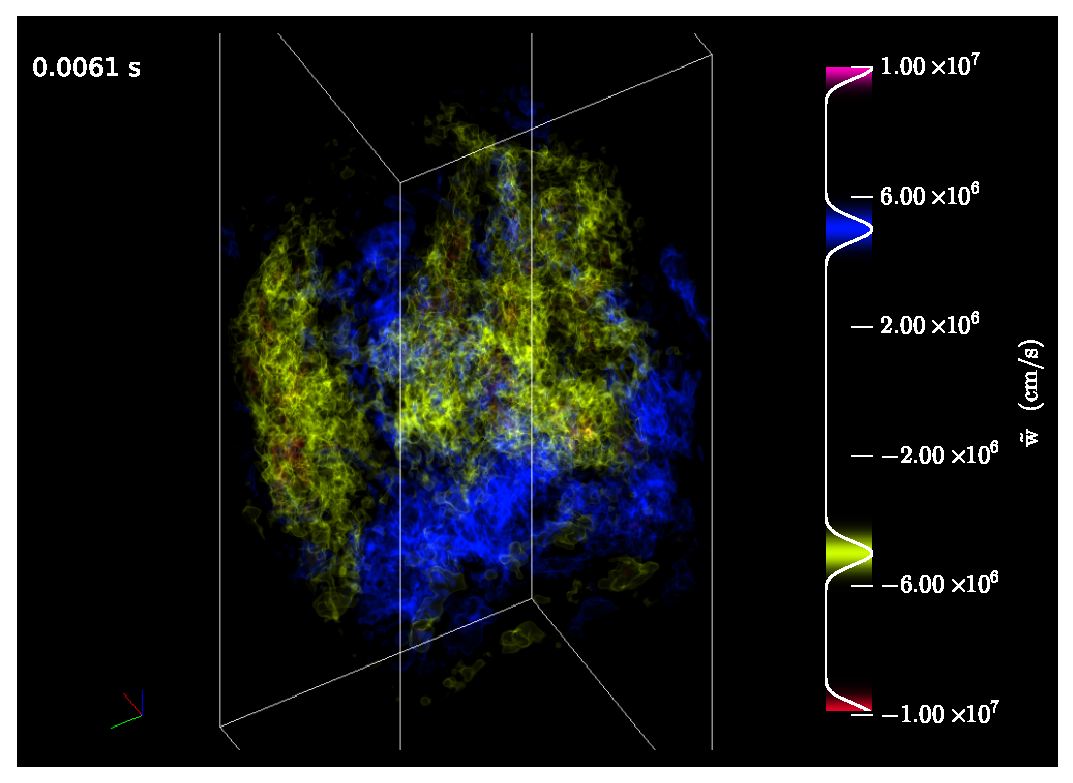
\includegraphics[width=0.42\linewidth]{xrb_vol_vz}
\hspace{0.25em}
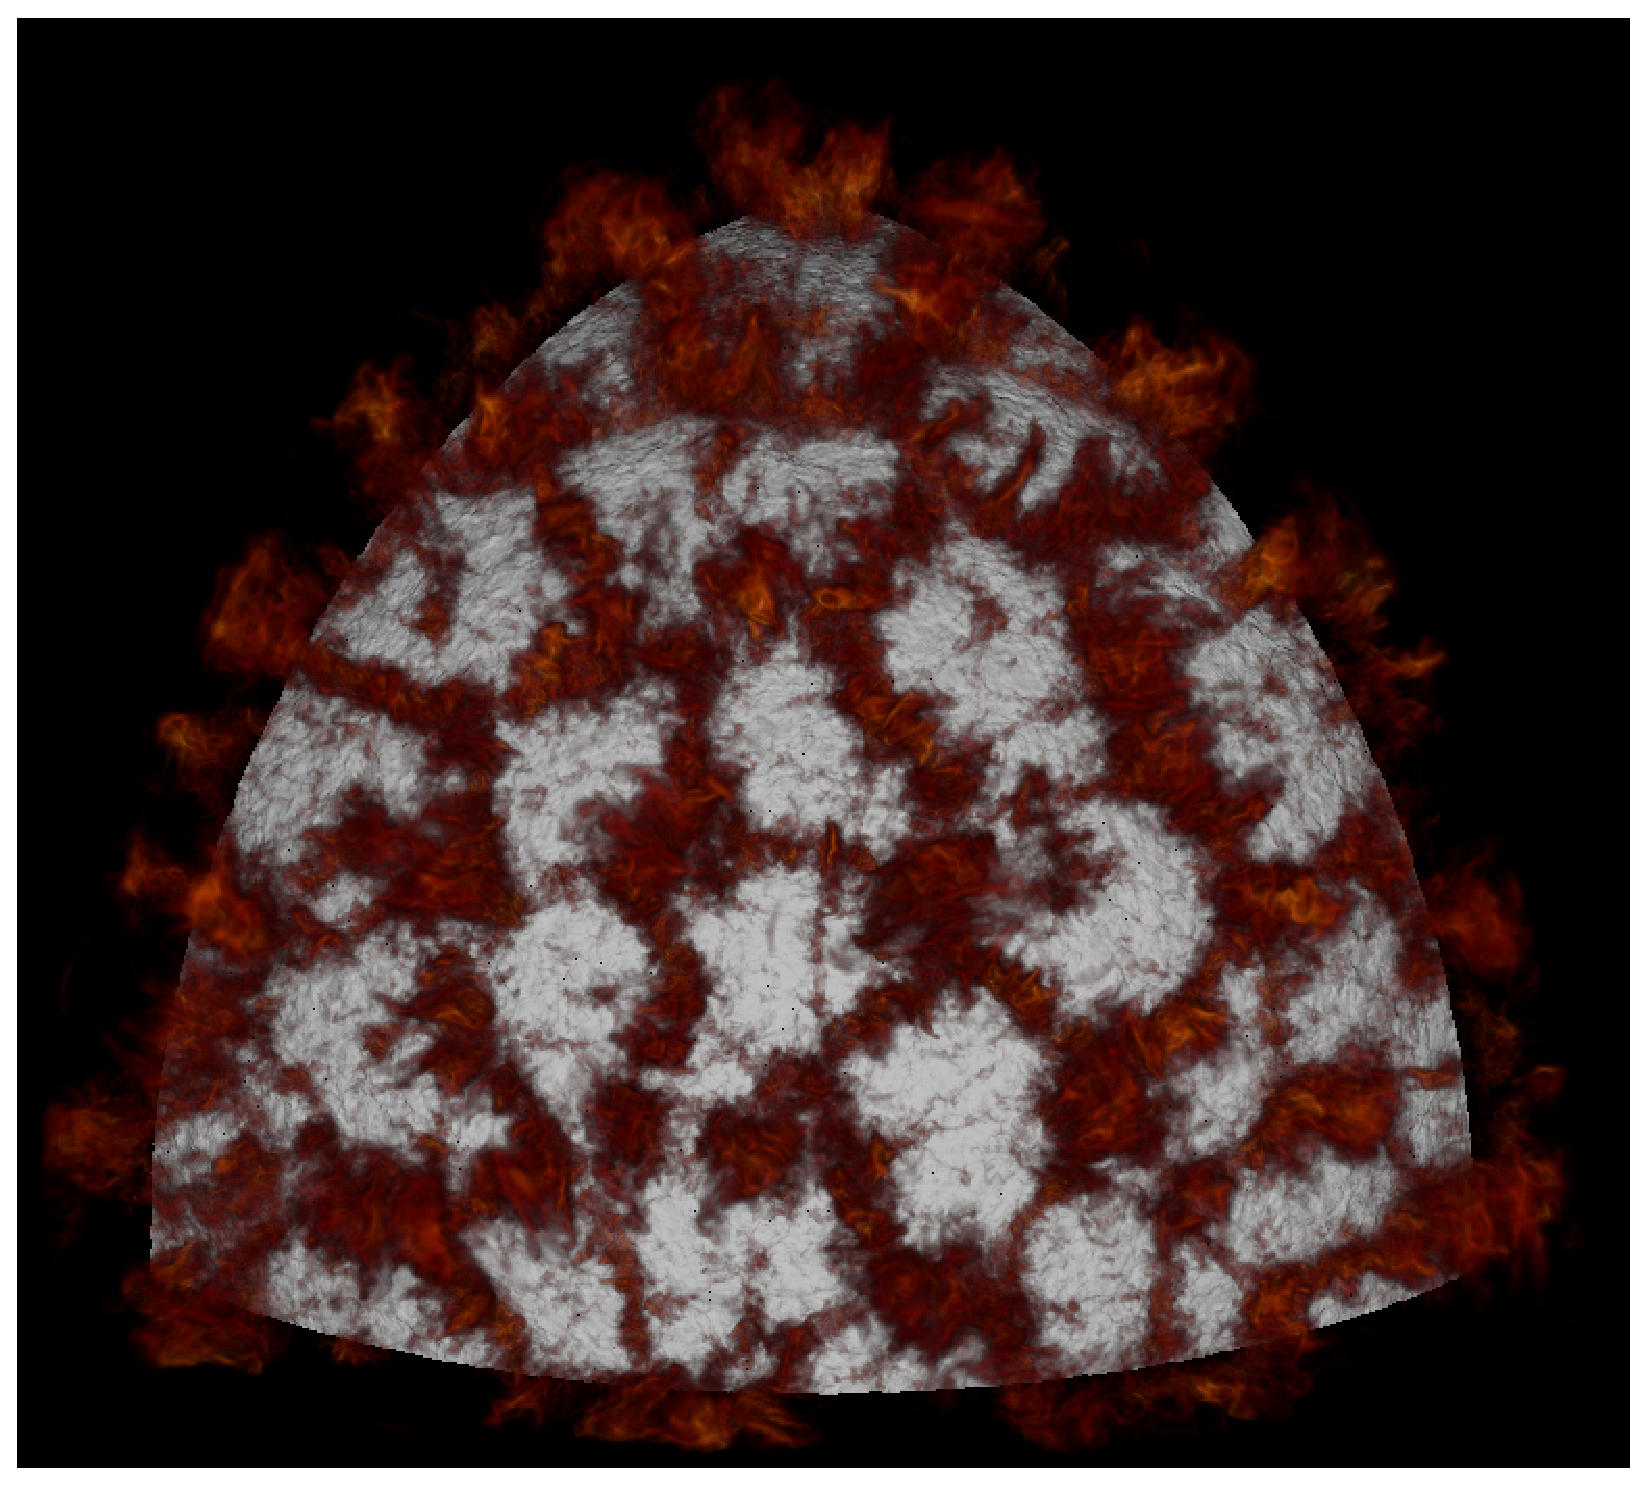
\includegraphics[width=0.32\linewidth]{ConvPlumes} \\[0.1em]
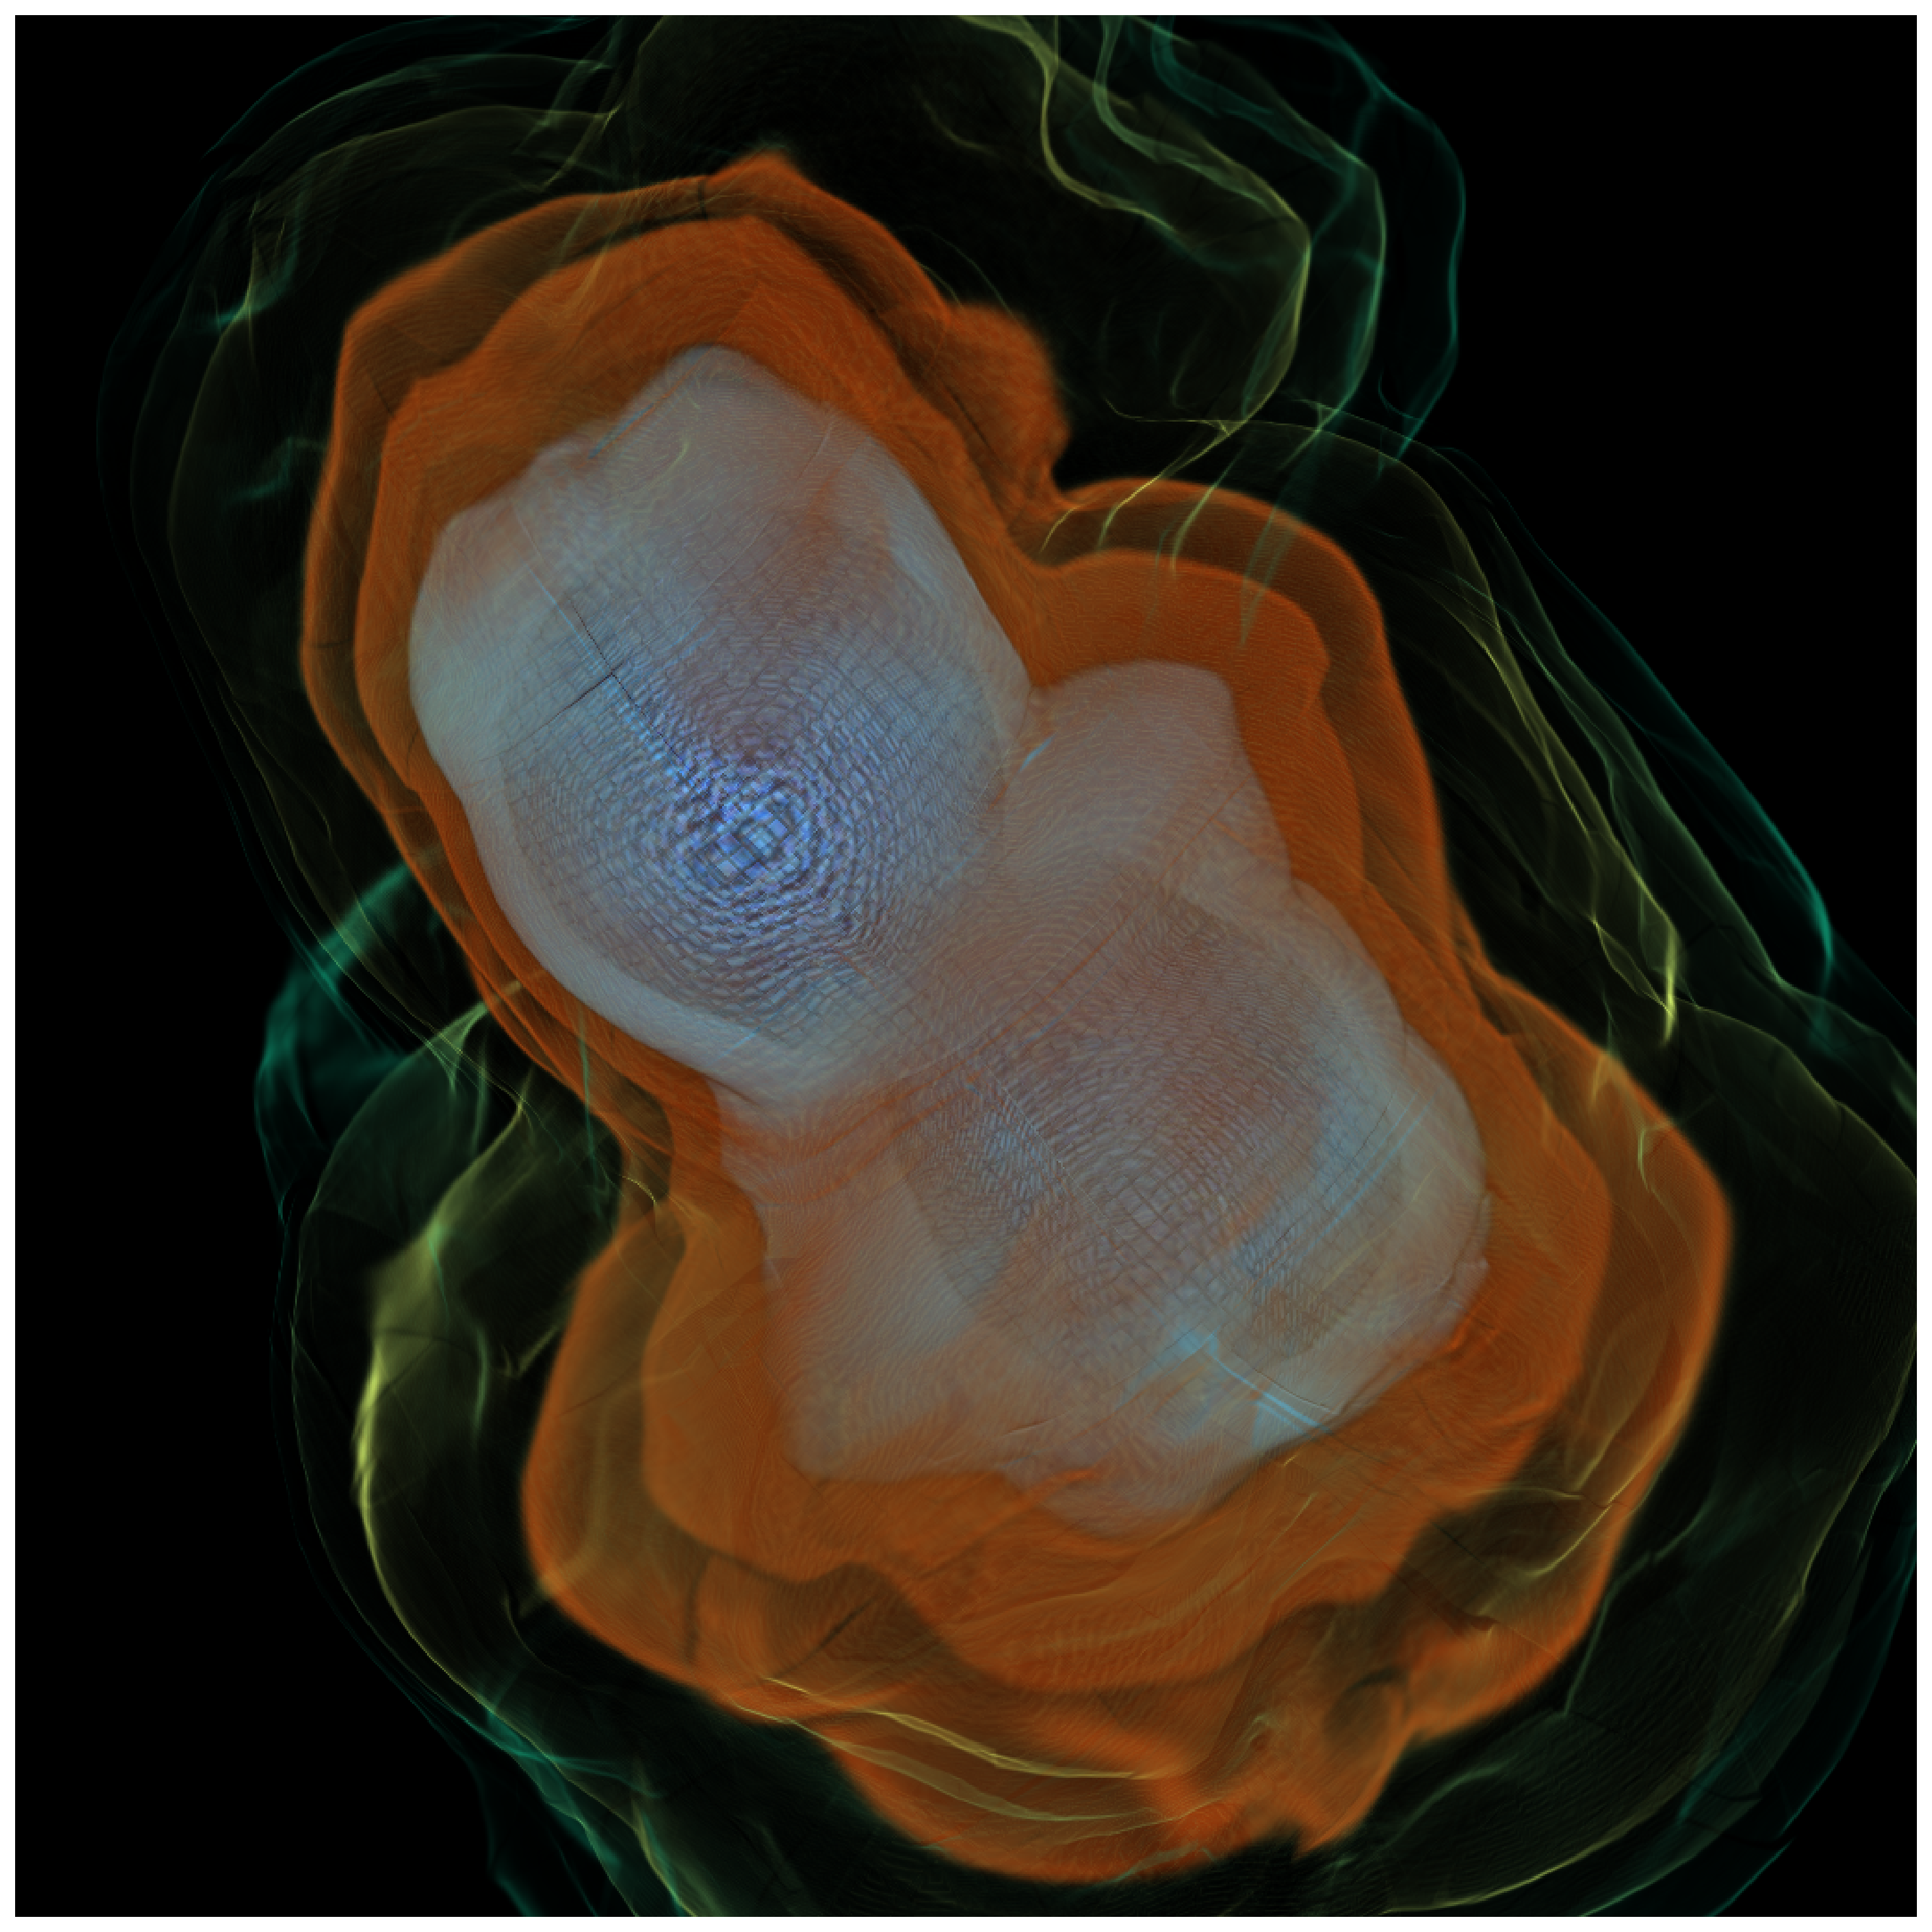
\includegraphics[width=0.3\linewidth]{generic3plt00180}\hspace{0.5em}
\begin{minipage}[b]{0.44\linewidth}
\caption{\label{fig:current-runs} (top left) Vertical velocity showing the
  convective structure in a \maestro\ XRB calculation.  (top right)
  Convective plumes in a \maestro\ sub-Ch calculation.  (left)
  Snapshot of a \castro\ simulation of the merger of two white dwarfs,
  with 0.90 and 0.81 solar masses. The contours represent density
  levels. The star on the upper left is disrupting and accreting onto
  the other star.}
\end{minipage}
\end{figure}


{\bf XRB simulations}:  Figure~\ref{fig:current-runs} shows
a snapshot from a current \maestro\ XRB simulation.
Our
2D study~\cite{XRB2} showed us that in order to resolve the 
nuclear burning, we needed to use a model with 6 cm resolution.
The current 3D simulation is done on a 256$\times$256$\times$768
grid.  At this resolution, we achieve timesteps of about $0.3~\mathrm{\mu s}$,
and this running this calculation to 0.1~s would require about 2 Mh on titan.

There two are primary goals for the XRB simulations.  First, we want to run
larger domains.  When the domain is small, the boundaries confine the convective
rolls, and an artificial flow is setup.  We want the width of the domain to be
several times larger than the scale height ($\sim 10$~m).  Keeping the
resolution fixed at 6~cm, we will perform simulations in 30~m and 60~m wide
domains.  These will give a clear picture of the dynamics of the convection
and allow us to answer the questions posed in the previous section:
how does the convection alter the nucleosynthesis? and are ashes brought
up to the surface where they can change the observables?

Secondly, we want to enable even larger domains by relaxing the
resolution requirements.  Using the results from years 1 and 2, we
will work on developing a sub-grid burning model that can be used to
capture the dynamics of the convection at coarser resolution.  We will
then push the domain sizes to 100s~m.  At this point, we can find ourselves
with burned regions in one part of the domain and unburned in others.  
Describing these different vertical structures is not currently possible
in \maestro\ (the different temperatures and composition result in different
hydrostatic structures, and \maestro\ is built on modeling the flow superposed
on a hydrostatic background).  Nevertheless, allowing for lateral gradients is 
in the plans for \maestro's development, and we hope to be in the position
to capture this new dynamics by year 3.

For the year 1 and 2 calculations, the resolved nuclear burning will require
us to use accurate reaction networks.  At the moment, we use a 10-isotope
network that captures the hot-CNO H burning, 3-$\alpha$ He burning, and some
links to heavier elements and the rp-process.  Our current study showed that
approximations in the network introduce some artifacts in the convective flow,
so we will push to larger networks.  As described later, we will ultimately
use the GPUs to offset the computational demands of these larger networks.


{\bf sub-Ch simulations}: \maestro\ sub-Ch convection simulations are
running on titan through our INCITE allocation right now (see
Figure~\ref{fig:current-runs}).  Our goal in the proposed INCITE
allocation is increased realism.  This means better initial models,
better nuclear physics, and following the event from convection to
ignition to explosion.  In~\cite{Zin13}, we modeled a single WD mass
(1 solar mass) and single He layer mass (0.05 solar masses).  Our 
current simulations are exploring an array of WD masses (0.8--1.2 solar masses)
and He masses (0.025--0.1 solar masses).  At the moment, we are relying
on simple parameterized models, and many of our simulations are done in an
octant, to reduce the computational cost.

Our proposed models will all be full-star.  When running in an octant,
boundary effects can lead to heating at the walls, perhaps biasing the
ignition.  Full star models avoid this issue.  These models rely on the AMR
capability in \maestro\ to focus the resolution in the He layer (we
model the entire star on a Cartesian grid).  Our current simulations
show that some mass configurations need increased resolution, so we will
explore higher resolution models in year 1. 

The current models include only the 3-$\alpha$ reaction and
$^{12}\mathrm{C} (\alpha,\gamma){}^{16}\mathrm{O}$.  We will use more
extensive networks in year 2.  Again, the GPUs will be needed here to allow
for this new physics.  At the same time, we will begin to
explore more realistic models from the MESA stellar evolution code.
These models will continue into year 3.  As development of \maestro\
continues, we aim to have the ability to do moderate rotation.
The issue here is that rotation deforms the star and there is no
longer a single 1D hydrostatic base state that describes the underlying
star.  We have ideas on how to improve this allowing for moderate rotation.
This development will take place over the next few years and we hope to
have the first applications of it in year 3 of this proposal.

A final effort will be to carry the convective calculations into the
explosive phase by restarting a promising model in \castro.  We have
done this process for the Chandra models of SNe Ia~\cite{Mal14}.  This
will be the first ``end-to-end'' simulation of the sub-Ch model for
SNe Ia.  It will be the most realistic such model to date and we expect
to learn a lot about the feasibility of the sub-Ch paradigm through
this calculation.




{\bf WDWD simulations}: Our simulations of merging white dwarfs are just
beginning.  We have modified \castro\ to incorporate the necessary physics
to allow for the simulation of the inspiral and merging.  In particular,
we extended the gravity Poisson solver to incorporate boundary conditions 
corresponding to an isolated potential.  To conserve angular momentum, 
we perform the simulation in the co-rotating frame---the
stars initially will appear motionless.

Our initial set of simulations map two WDs onto the computational
domain.  For simplicity, these WD models were constructed in isolation
with a uniform composition.  After a few orbits tidal forces
deform the stars and when the stars are close enough, the lower mass
star can be disrupted and the material will accrete onto the more
massive star (see Figure~\ref{fig:current-runs}).  In year 1, we will explore
a variety of different mass ratios and focus on understanding what happens
when the disruption occurs and material first hits the more massive star.
In particular, we wish to see if the conditions necessary for the detonation
of the carbon fuel are met.

In year 2 we will refine the simulations by incorporating a nuclear
reaction network.  This will allow for us to self-consistently model
the merger event beyond the time when they first touch.  We will also
begin to use self-consistent initial conditions.  These are
equilibrium conditions that initialize the stars on the grid as a
system, so the tidal-distortion effects are already in place.  This
reduces the cost of the simulation by allowing us to model fewer orbits
before the merger.

There are a lot of unknowns in the WDWD system, and we will use the
INCITE time to explore the parameter space.  We will consider many
different initial configurations and explore the resolution needs for
these simulations.  With AMR, we can focus the resolution on the
conditions where the detonation may take place, saving on the
computational cost.  In year 3, we will explore models with initial
conditions generated from a stellar evolution code like MESA.  These
may not have uniform composition and perhaps will have a thin helium
layer on the surface, both of which can alter the nuclear burning.


{\bf Post processing and observables}:  
%
For the SNe Ia models that we bring to explosion, we will use the
\sedona\ radiation transfer code to produce synthetic observables
(lightcurves and spectra)---the \sedona\ author Dan Kasen is a Co-I on
this proposal.  This post processing was done with many of the explosion 
models in the current INCITE allocation and the pieces are in place for this
workflow. We do not expect \sedona\ to require a lot of compute
time for these models.


{\bf Exploratory simulations}:
%
We are
capable of modeling all phases of these explosive phenomena.  As a
result, when a new idea is promoted in the field, we will be in an
excellent position to explore it through detailed high-resolution
simulation.  We will keep pace with the field and propose some add-on
calculations in later year renewals.  One example already placed in
our milestones is the URCA calculation.




%-----------------------------------------------------------------------------
\section{COMPUTATIONAL READINESS}



%% Proposals will be assessed on the need for, readiness to use, and
%% reasonableness of the request for resources. {\bf This section is
%%   typically about 5 pages.}

The proposed work uses two simulation codes: \maestro, a low Mach
number hydrodynamics code suited to convective flows and \castro, a
compressible hydrodynamics code designed for high Mach number flows.
The two codes share a common framework, built around the
\boxlib\ library.  We note that both of these codes are freely
available to the community and any improvements to their parallel
performance based on the work proposed here will benefit all users of
the codes.  The unique features of titan, in particular the GPUs on each
node, are of critical importance to meeting the science goals proposed here---GPUs,
will allow us to consider bigger networks. 
We have proof-of-concept GPU results on titan already, and discuss our plans
for finishing the implementation below.


\subsection{Use of Resources Requested}

%% Describe your proposed production simulations and state how the runs
%% are tied to each of your project's goals and milestones (the Milestone
%% Table). For the simulations you plan to carry out during production
%% runs, provide a
%% \begin{enumerate}
%% \item description of what jobs are going to be run and how they relate
%%   to the research/development objectives given above;
%% \item description of processor/core use for large runs (e.g.,
%%   10,000-hour run with 100 cores, or ten 10-hour runs with 10,000
%%   cores, for a 1,000,000-hour allocation);
%% \item clear, detailed explanation as to how you calculated the
%%   requested number of processor hours; and
%% \item summary of your anticipated annual burn rate (e.g., linear or
%%   with periods of peak usage).
%% \end{enumerate}
%% \vspace{-.2in}

Our list of large jobs to run along with detailed time estimates is given in
the previous section.  In each case, the time estimates
were computed based on actual runs of the proposed problem on titan.
The convection jobs all share something in common---the need for long
time-integration.  This means {\em many} trips through the queue (it's
not uncommon to require 500 wallclock hours, broken up into may
smaller segments).  With 10,000 cores, this is 5~Mh---a number
representative of many of our jobs.  This will represent the typical
job size for the base calculations.  The addition of bigger networks
will push the base calculations up to larger core counts in subsequent
years.

There are several large calculations each year when that will need more
processors.  The biggest XRB runs will require 10,000s of cores.  We
scale well to that point now, and planned developments described
below will make this a more typical size.  For the WDWD simulations,
as the stars merge, the number of AMR grids created will dramatically
rise, as a result, the last 10\% of the simulation may require
10$\times$ more processors.  The same will be true of the
\castro\ continuation of our \maestro\ sub-Ch model.

Our usage throughout the year will have periods of intense
usage---when we have decided on our initial conditions and are running
a suite of calculations for a paper.  Many of us teach, and will be
less active during the semester, but the graduate students will be running
steadily throughout the year.


\subsection{Leadership Classification}

The job characteristics as described above are hundreds of hours on
10k cores for our standard jobs and several 10,000s of cores (again
for hundreds of hours) for our biggest jobs.  We are proposing 10s of
jobs per year, with an average cost of a few Mh, and the biggest jobs
requiring 25 Mh.  These numbers cannot be met by any facility other
than through INCITE.  We can run at this scale today.  Any larger, and
it becomes difficult to get the runtime needed to complete our jobs.
Our largest jobs will be on the leadership class by themselves,
requiring $\sim 20$\% of the machine, and our wide range of concurrent
moderately-sized studies for the proposed simulations will utilize
more than 20\% of the total machine.  Finally, we have been investing
our time in porting our microphysics to the GPUs.  This is essential
to implementing the physics we require.  A proof-of-concept
running on titan is shown below.  This will speed up some of the more
time-intensive parts of our simulations and enable new science (in
particular, bigger reaction networks).  For this investment to payoff,
we need a machine with GPUs on all of the nodes---titan has been our
target.  Only INCITE resources meet these needs.

%% Summarize the requirement that best exemplifies the proposed
%% computational work. Leadership targets in the INCITE program typically
%% include one or both of the following categories:

%% \begin{enumerate}
%% \item Use of 20 percent or more of the system for production
%%   simulations. Parameter sweeps, ensembles, design of experiments, and
%%   other statistical methods that require large numbers of discrete or
%%   loosely coupled simulations may be considered capability-class
%%   campaigns. See the FAQS <link> for details and qualifiers.
%% \item Specific architectural needs that can only be met by the LCF.
%% \end{enumerate}

%% 20 \% of titan is currently about 3738 nodes (59,808 cores + GPUs)...

\subsection{Parallel Performance}

%% Provide direct evidence, {\bf including supporting quantitative data},
%% for your production application's parallel performance for the
%% intended research simulations. Ideally, the proposing team will have
%% generated the data. If you cite work by others, explain why it is
%% applicable here. You should use the application code you intend for
%% the production work, not a related code. Data for sample systems not
%% related to the intended research is undesirable. Performance
%% benchmarking should reflect all I/O requirements. Parallel performance
%% data in either strong or weak scaling mode must be provided. Explain
%% how the strong or weak scaling applies to the proposed work. See the
%% examples at the end of this document.

\begin{figure}[t]
\centering
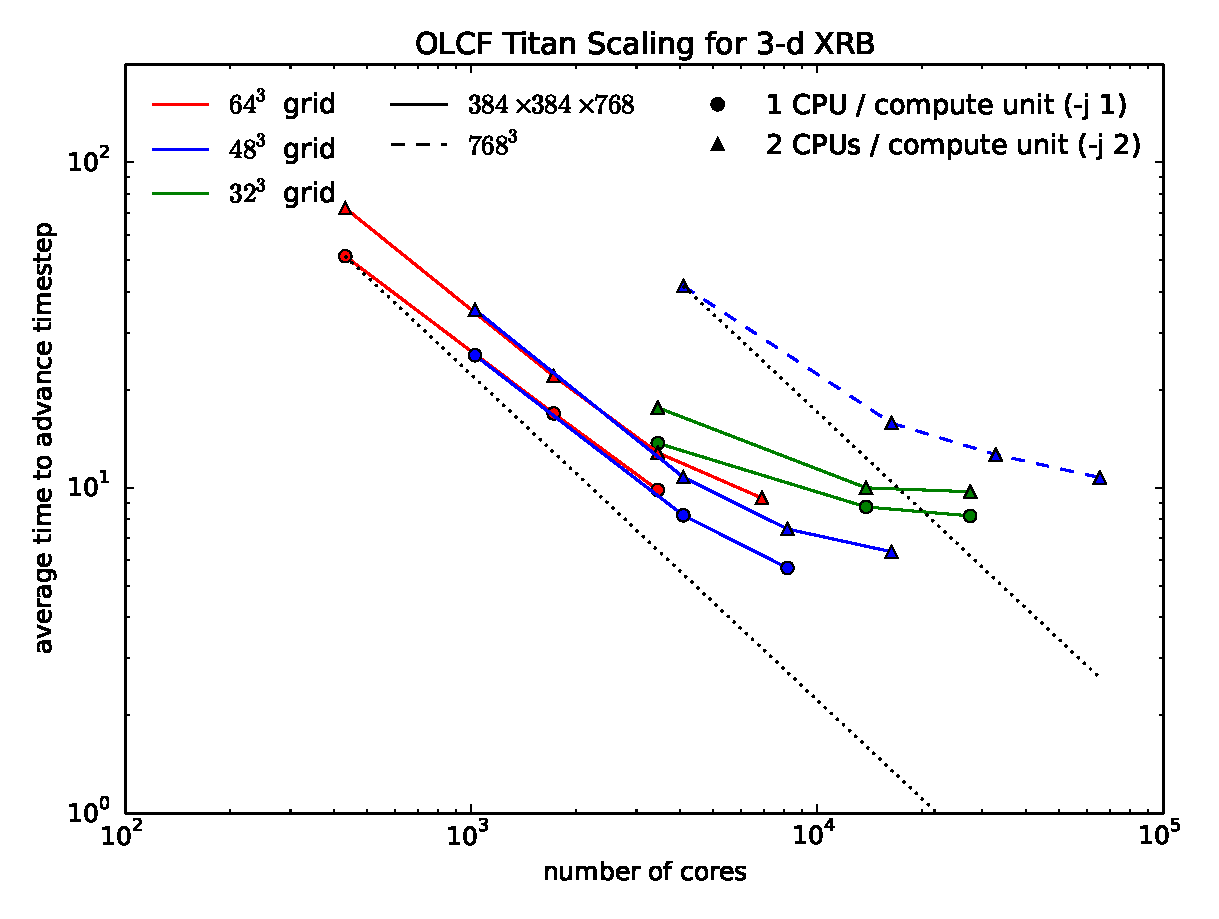
\includegraphics[width=0.49\linewidth]{xrb_titan_scaling_by_grid}
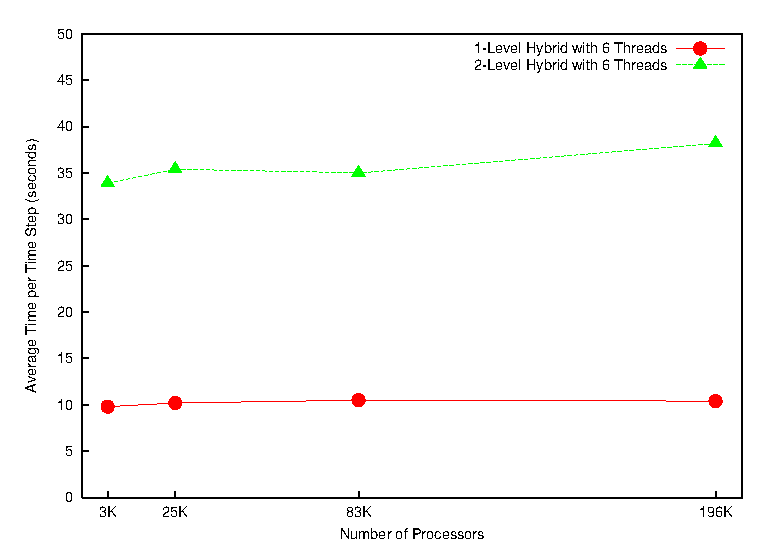
\includegraphics[width=0.49\linewidth]{castro_scaling} \\[0.5em]
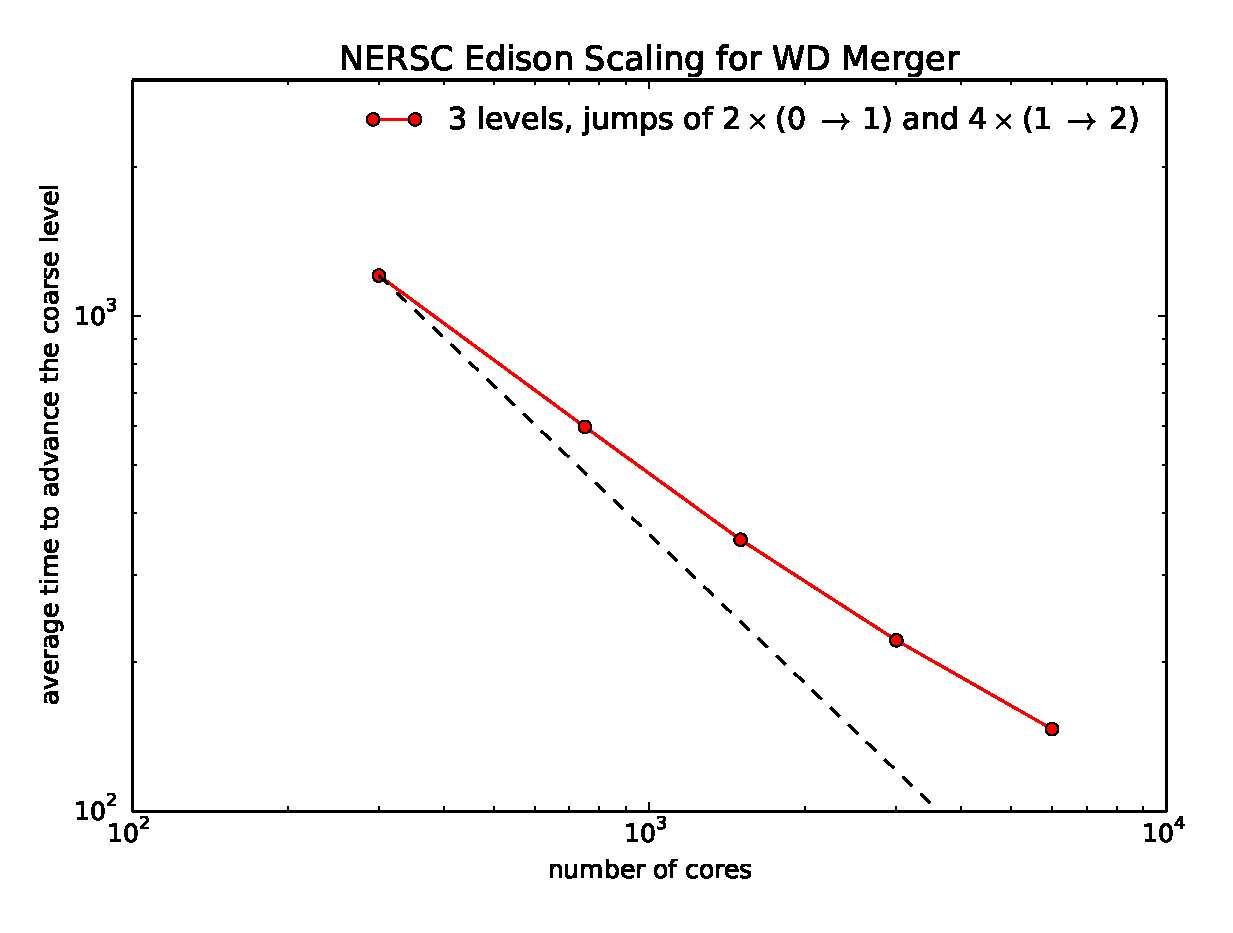
\includegraphics[width=0.49\linewidth]{edison-wdmerger-scaling.eps}
\begin{minipage}[b]{0.5\linewidth}
\caption{\label{fig:scaling} (top left) \maestro\ strong scaling for
  the XRB problem.  Two problem sizes are shown, with 
  different domain decompositions and OpenMP
  threads.  In each case, the time to advance the solution is the
  average of 10 steps.  Comparing the two problem sizes shows the weak
  scaling.  (top right) \castro\ weak scaling on the titan-predecessor
  jaguarpf for a SNe Ia explosion.  This has the same physics and
  solvers as will be used for the sub-Ch explosions. (left)
  \castro\ strong scaling for the initial (non-interacting) stage of
  the WDWD problem, run on the NERSC Edison machine.  This solves the
  full Poisson problem using multigrid with isolated boundary
  conditions.}
\end{minipage}
\end{figure}

%% In year 1, the majority of our jobs will use \maestro, so we focused in
%% detail in obtaining real-world scaling numbers on titan for the main
%% year 1 jobs.

{\bf \maestro}:
%
Figure~\ref{fig:scaling} (top-left) shows the strong scaling
behavior for our \maestro\ XRB problem on titan.  A subset of
this same information is shown in a speedup plot as well (Figure~\ref{fig:speedup}).
For \maestro\ strong
scaling, we explored two problem sizes (a 3D XRB with a domain
of 384$\times$384$\times$768 zones, and one that is twice as wide in
each lateral direction, $768^3$).  For the smaller size, we did three
different domain decompositions---breaking it up into 432 $64^3$
sub-grids, 1024 $48^3$ sub-grids, or 3456 $32^3$ sub-grids (the
different color lines show these different decompositions).  We always
assigned one grid per MPI task and experimented with 1, 4, 8, or 16
OpenMP threads per MPI task.  We also explored the number of CPUs per
compute unit (since two titan CPUs share a single floating point unit
in the compute unit).  We find that only using one CPU per compute
unit results in about a 30\% performance gain, but it does not affect
the scalability.  We see that we get the best scaling with the larger
sub-grids ($64^3$ and $48^3$), and that $32^3$ does not thread well
for our application.  Furthermore, we see that with the large grid
sizes, we get good strong scaling over a decade increase in processor
count.  Note, we did not explore assigning tasks to specific NUMA nodes
in this test.  Finally, it seems that using 16 threads incurs a slight performance
penalty over lower thread counts.  

For the bigger job, we only did a single decomposition ($48^3$ grids)
using all CPUs on the compute units.  This run has $4\times$ as much
work and is run on $4\times$ the number of processors as the
corresponding smaller job.  Looking at the first point in the curve
and comparing to the corresponding point in the smaller-job-size
curve, we see that we have excellent weak scaling as we increase the
job size.  The strong scaling curve for this larger problem
 shows that \maestro\ is reaching up to effective use
of 20\% of the machine.  Some of the XRB runs in year 2 will be larger
domains still.

\begin{figure}[t]
\centering
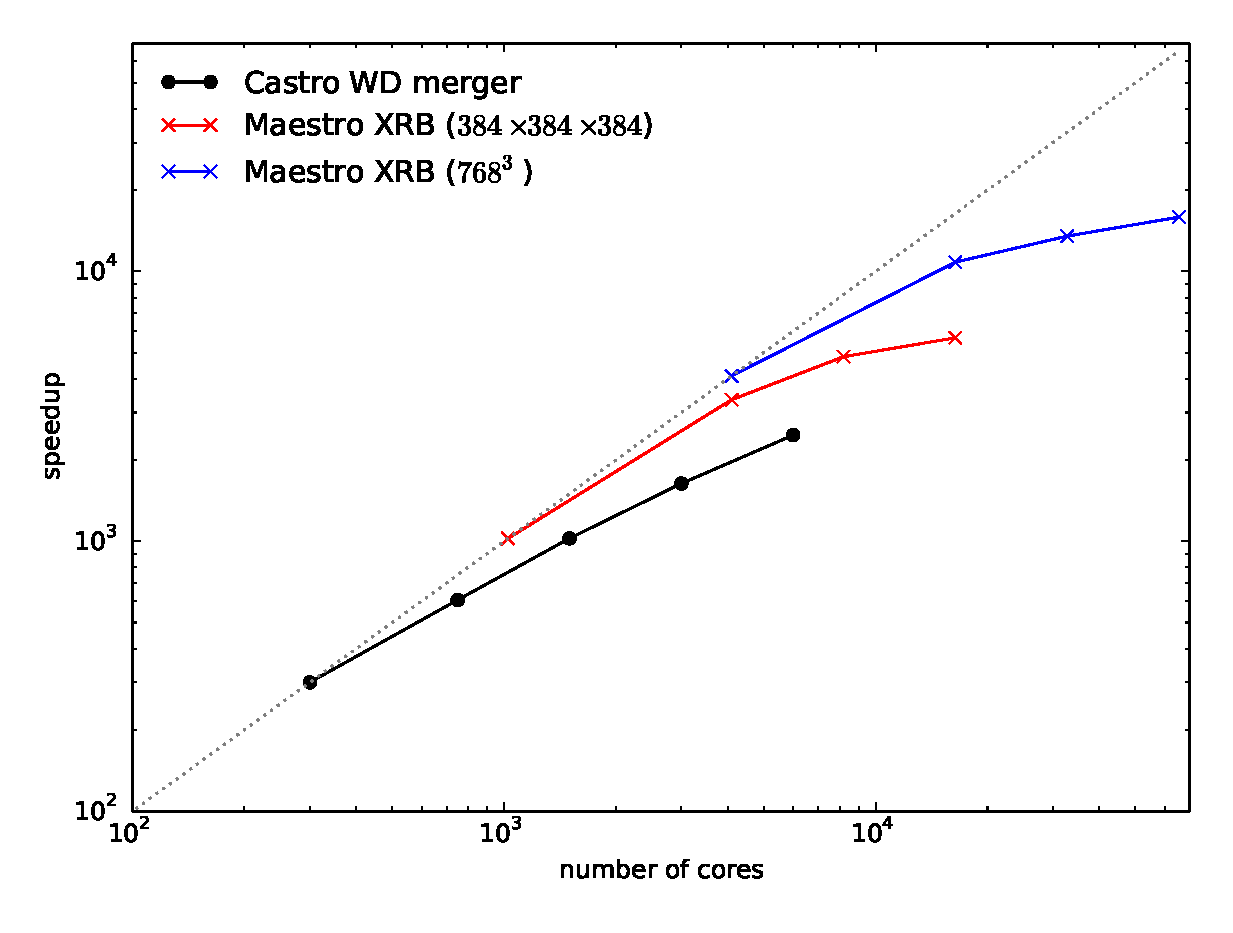
\includegraphics[width=0.48\linewidth]{speedup}
\begin{minipage}[b]{0.5\linewidth}
\caption{\label{fig:speedup} Speed-up plot for the \maestro\
and \castro\ strong scaling data.  For the \maestro\ runs,
we only show the $48^3$ grid case using all CPUs on a compute
unit (-j 2)}
\end{minipage}
\end{figure}

The low Mach number constraint in imposed through a divergence
constraint on the velocity field.
\maestro\ uses two different multigrid solvers in the algorithm to
enforce this constraint.  At
the half-time, a cell-centered multigrid solver enforces the low Mach
divergence constraint on the velocities that go into the fluxes.  At
the final time, a node-centered (nodal) multigrid solver enforces
this constraint on the final velocity field.
Finer-grained timers tell us that the main scaling bottleneck is in
the nodal multigrid solver.  We have a plan to improve this scaling
that we expect to implement in the near future---we discuss it 
in section 3.5 below.  We note that this test corresponds to the 
proposed XRB simulations, which will run in exactly the fashion
tested here.  The sub-Ch and URCA \maestro\ simulations will exercise the
same parts of \maestro\ and we would expect similar scaling.  For
both problems, our plans have us increasing the reaction network in
later years---this will only improve scaling since the network is purely
local physics.

{\bf \castro}: For \castro, Figure~\ref{fig:scaling} (top-right) shows a
weak scaling study where we put a WD on the adaptive grid and
simulated hydrodynamics with self-gravity using a monopole
approximation---this is representative of the sub-Ch
\castro\ simulations proposed.  This was run on the pre-titan hardware
(jaguarpf).  We considered both a single level and a two-level case
where the coarse resolution is equivalent to the single level case.
Both scale well to approximately 200K processors.  We note that the
2-level case does approximately three times the work of the single
level case.  The data shows an overhead of approximately 15-20\% for
AMR; however, achieving the same resolution as the two-level
simulation with a uniform grid would be a factor of 16 more than the
single level example treated here.

Our scaling numbers for the WDWD problem consider the initial stage,
when the stars are not yet interacting.  This is shown in the bottom
left panel of Figure~\ref{fig:scaling} and in the speedup plot, Figure~\ref{fig:speedup}.
The calculations were run on the NERSC Edison
platform, a Cray machine that shares many characteristics with titan.
This problem uses 3 levels in the grid hierarchy, level 0 is $480^3$,
level 1 is $2\times$ finer than level 0, and level 2 is $4\times$
finer than level 1, giving us an effective grid of $3840^3$.  This is
typical of the size problem we will want to run.  Gravity is done
using a full Poisson solve with multigrid, with the isolated boundary
conditions constructed by doing a multipole expansion (up to $l=6$) on
the coarsest grid.  \castro\ and \maestro\ share the same
cell-centered multigrid solver from \boxlib, and our early numbers
show that the gravity solve with isolated boundary conditions takes
approximately 25\% of the runtime for a WDWD problem where the stars
have not yet begun interacting.  We scale for over a decade in core count.  At high core counts, we become work
starved---there are too few grids at the fine level to redistribute equally.  As the stars interact, many more grids will be created
(about an order-of-magnitude increase is expected), and this will
improve the scaling and allow us to move to higher core counts.  Our
plan is therefore to start this problem on a moderate number of cores
and move to larger core counts as it evolves.  The addition of burning
in year 2 will greatly increase the local physics, further improving
the scaling.



{\bf I/O}: 
%
We directly measured the time to output from
\maestro\ on titan, writing a 50~GB plotfile at a data rate
ranging from 4--12 GB/s.  We note that I/O takes less than 1\% of our
runtime, and it will not be an issue for the proposed runs.
As \castro\ uses a similar I/O strategy, we expect it to attain the
same performance.  All of our codes have checkpoint/restart capability 
to make effective use of titan's queue system.


\subsection{Computational Approach}

%% Provide a detailed description of your computational approach,
%% including a discussion of the state of the art in the field. The
%% description should also mention:

%% \begin{enumerate}
%% \item Particular libraries required by the production and analysis
%%   software, algorithms and numerical techniques employed (e.g., finite
%%   element, iterative solver), programming languages, and other
%%   software used.
%% \item Parallel programming model(s) used (e.g., MPI, OpenMP, Pthreads,
%%   CUDA, OpenACC).
%% \item Project workflow including the role of analysis and
%%   visualization; identify where the analysis will be done and any
%%   potential bottlenecks in the analysis process.
%% \item Software workflow solution (e.g., pre- and postprocessing
%%   scripts that automate run management and analysis) to facilitate
%%   this volume of work.
%% \item I/O requirements (e.g., amount, size, bandwidth) for restart,
%%   analysis, and workflow. Highlight any exceptional I/O needs.
%% \item Data storage requirements. Estimate anticipated cumulative size
%%   of stored data at the end of the requested award. What do you plan
%%   to do with the data at the end of the project? Do you plan to share
%%   the data or make it public? Do you have tools and/or plans to reduce
%%   the data? Justify data storage needs that exceed 1 petabyte.
%% \end{enumerate}

\maestro\ decomposes the fluid state into a 1D radial hydrostatic base
state and a perturbational Cartesian state.  A divergence constraint
on the velocity field captures the compressibility due to background
stratification and local heating/diffusion sources.  The resulting
system allows for much larger time steps to be taken compared to
corresponding compressible codes ($\sim 1/M$ larger), where $M$ is 
the Mach number.
The algorithm
\cite{multilevel} utilizes a second-order accurate approximate
projection method, developed first for incompressible flows.  Fluid
quantities are advected using an unsplit Godunov method, with
reactions incorporated via operator splitting.  The provisional
velocities are then projected onto the space that satisfies the
divergence constraint.  The projections involve elliptic solves,
solving a variable-coefficient Poisson problem,
computed using a multigrid algorithm.  AMR is
used to achieve high spatial resolution.  \maestro\ is written primarily
in Fortran 95 and is parallelized using MPI and OpenMP.  It is highly
portable, and regularly runs at the OLCF, NERSC, and NCSA.

\castro~\cite{castro} is based on a compressible flow formulation in
Eulerian coordinates and includes self-gravity and reaction networks.
All \castro\ calculations will use AMR on a 3D Cartesian grid.  The
hydrodynamics in \castro\ is based on the either unsplit piecewise
linear (PLM) or piecewise parabolic method (PPM)~\cite{ppmunsplit} and
is designed to work with a general convex equation of state.
\castro\ supports Newtonian self-gravitational forces through either a
simple monopole approximation or a full solution of the Poisson
equation using geometric multigrid techniques.  The approach to AMR in
\castro\ uses a nested hierarchy of logically-rectangular grids with
simultaneous refinement of the grids in both space and time.  The
integration algorithm on the grid hierarchy is a recursive procedure
in which coarse grids are advanced in time, fine grids are advanced
multiple steps to reach the same time as the coarse grids and the data
at different levels are then synchronized.  The synchronization for
self-gravity is similar to the algorithm introduced by
\cite{miniati-colella}.  

Both \maestro\ and \castro\ uses a hybrid
programming model based on MPI and OpenMP.  Distribution of grid
patches to nodes using MPI provides a natural coarse-grained approach
to distributing the computational work, while threading of loops over
zones in a grid using OpenMP provides effective fine-grained parallelization.
Both codes use the same interface to the EOS and 
thermonuclear reaction networks.  This enables us to
switch from a low Mach number simulation with \maestro\ to a fully
compressible simulation using \castro\ without changing the underlying
physics.  

For analysis, \maestro\ and \castro\ dump out global
diagnostics at each time step and plotfiles at regular intervals.  The
visualization packages \visit\ and \yt\ have native support for the
\boxlib\ file format.  We expect the largest simulations
to output about 100--200 TB each in plotfiles, putting the storage needs at about
800 TB in year 1, rising to 1 PB in year 3.  We will save plotfiles for as long as needed to finish the
analysis and publication of the results.  Only a minimal set of checkpoint
files will be archived.  Where possible, we will store output in single precision
to conserve space.



\subsection{Developmental Work}

Both \maestro\ and \castro\ already scale well on titan and are
capable of running the proposed science.  Nevertheless, we are
continually working on the performance of these codes, and in
particular, in the last year have been actively targeting titan and
its GPUs.  Our graduate students have been the lead on this effort.

%% For the computational approach above, describe what, if any,
%% development work has been carried out to date, especially on the
%% architecture of the requested resource. Describe what development work
%% will be executed, and when, during the proposed INCITE campaign.

%% The current bottleneck in \maestro's threading performance is in the
%% smoothing during the nodal multigrid solve.  Whereas the cell-centered
%% solve uses a standard 7-point stencil for the Laplacian, which can be
%% solved using red-black Gauss-Seidel smoothing (parallelized with
%% OpenMP on a grid), the nodal solve requires a dense stencil for
%% algorithmic reasons.  This dense stencil cannot be decomposed in a
%% red-black fashion, and more complex decompositions have shown worse
%% performance.  Other alternatives like Jacobi smoothing do not converge
%% well in the algorithm.  In the next year, we will research and
%% implement an alternative, Chebyshev smoothing, which has been shown to
%% parallelize well~\cite{smoother}.  We believe that this will eliminate
%% the OpenMP bottleneck.  This work will be done in collaboration with
%% the \boxlib\ developers.

Our codes use multigrid algorithms that iterate across a hierarchy of
grids of different resolution. At coarser levels of the multigrid
hierarchy, the relaxation schemes that form the core of the multigrid
algorithm may not be able to effectively utilize high thread counts
because communication costs will dominate floating point
work. Furthermore, standard relaxation schemes for denser stencils
such as the nodal solver in \maestro\ are not well suited to high thread
counts. We are pursuing a number of possible strategies for dealing
with this issue including relaxation schemes with higher floating
point intensity but good thread performance, communication avoiding
algorithms and hybrid strategies that limit the amount of coarsening
to address these issues.  This effort is led by the \boxlib\ group.

%% Our current development efforts are focusing on efficient use of the
%% GPUs on Titan. \castro\ and \maestro as originally released, being
%% based on the \boxlib\ framework, were designed for hybrid parallelism
%% on CPUs with MPI and OpenMP. The design is such that porting to GPUs
%% is natural. The directive approach of OpenACC means that a
%% straightforward approach for us is to take loops that were previously
%% threaded with OpenMP, move the relevant data to the GPU in an OpenACC
%% data region, and execute the loop on the accelerator. Since these
%% codes are designed in a modular fashion, our development model
%% involves taking the various microphysics modules and refactoring them
%% so that they can be parallelized with OpenACC directives. To date, we
%% have begun this work on two of the modules.

With the advent of OpenACC 2.0 (in particular, its ability to support
function calls), we have begun porting the microphysics (EOS,
reactions) in our codes to the GPUs on titan.  The EOS is the most
time-consuming standalone physics module for the WDWD problem.  Both
codes use the publicly available Helmholtz stellar EOS, which although
itself can take a vector, it was originally structured in our codes to
work on a single zone at a time.  We converted the EOS to operate in
vectorized fashion, and moved almost all of the logic inside the main
EOS routine, to maximize the work done in one place. This EOS
calculates the relevant thermodynamic quantities by interpolating from
a table that is read into memory at the beginning of the
calculation. We used the OpenACC 2.0\, \texttt{enter data}\, construct
to move this table onto the GPU at the beginning of the simulation,
and have it reside there for the remainder. Then we implemented a
parallel loop over the input vector for the main EOS routine. To check
the performance gain, we wrote a driver routine that loads the table
into memory and then executes a number of EOS calls. We compared this
to an OpenMP parallelization of the same loop. We chose a vector size
of $32^3$---representative of the size of a typical AMR grid that will
enter the EOS routine.  For low numbers of calls, the time of
execution is dominated by the table read, but for large numbers of
calls (approaching what we would see in a production run), the loop
parallelized by OpenACC is significantly faster than OpenMP, as in
Figure \ref{fig-eos-openacc}.  We have run some actual Castro
exploratory WDWD calculations using the OpenACC EOS.  For a $256^3$
uniform grid on 512 nodes, running for 10 timesteps, the case with the
OpenACC EOS runs 60\% faster than an unthreaded implementation of the
EOS.  We are still optimizing, but this shows that the EOS is a large
factor in this problem's runtime, and we are able to run a Castro simulation
using the GPUs on
titan today.



\begin{figure}[t]
  \centering
  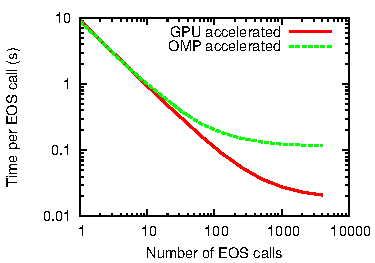
\includegraphics[width=0.5\linewidth]{eos_openacc.pdf}
  \begin{minipage}[b]{0.45\linewidth}
  \caption{Comparison of OpenACC (solid, red) and OpenMP (dashed,
    green) parallelizations of the EOS. Each calculation involves
    reading the EOS table into memory and then calling the EOS a
    certain number of times. The vertical axis shows the average time
    per call.  With few calls the execution time is dominated by
    reading the table into memory, but this is amortized out as we
    call the EOS more.  The OpenACC-threaded calls are significantly faster
    than the OpenMP-threaded calls, even when taking data movement to
    the GPU into account.\label{fig-eos-openacc}}
   \end{minipage}
\end{figure}

We are applying similar techniques to put our reaction networks on the
GPUs.  For our XRB simulations, the reactions can represent a
significant fraction of the runtime (up to 25\% with our current,
small network).  Furthermore, we wish to use much larger networks to
better capture the nucleosynthesis and energetics of the burning.  To
facilitate this, we are in the process of changing the ODE integrator
in \maestro\ from VODE to a vectorized implicit ODE integrator written
by our colleagues at LBNL.  This will allow us to call the reaction
network for a vector of zones and to put this entire operation onto
the GPUs, much as we did for the EOS.  We expect to finish this work
in the next month or two.  We note that a similar procedure of
offloading the reactions to GPUs has been taken by other codes running
on titan (the Chimera core-collapse code~\cite{chimera-gpu} and the
S3D combustion code~\cite{s3d}) and we have begun to make contact with
our OLCF liaison about the strategies needed here.

Finally we note that the porting of the microphysics to GPUs described
here applies to both \maestro\ and \castro, and furthermore, we will
make all of the resulting improvements available to the community.
Importantly, accelerated microphysics opens the door to new physics.
The network modifications will allow us to use larger, more realistic
reaction networks.  The GPU version of the EOS will allow us to 
``undo'' some of the common approximations used in hydrodynamics 
codes to avoid expensive EOS calls~\cite{colellaglaz:1985}, and improve our thermodynamic
consistency.

\bibliographystyle{unsrtnat}
\bibliography{refs}




\end{document}
